\section{Sucesiones de funciones}

\begin{definition}[Convergencia puntual]
  Sean $X \subset \R$ y $f_n\colon X \to \R$ para cada $n \in \N$. La sucesión ${(f_n)}_{n \in \N}$ \emph{converge puntualmente} a $f\colon X \to \R$ si para todo $x \in X$,
  \[
    \lim_{n \to +\infty} f_n(x) = f(x).
  \]
\end{definition}

\begin{eg}
  Las funciones $f_n\colon [0, 1] \to \R$, $f_n(x) = x^n$, convergen puntualmente a la función $f\colon [0, 1] \to \R$ dada por
  \[
    f(x) = \begin{cases}
      0 & \text{si } 0 \leq x < 1, \\
      1 & \text{si } x = 1.
    \end{cases}
  \]
  En efecto, si $x \in [0, 1)$, $\lim_{n \to \infty} x^n = 0$, y si $x = 1$, $\lim_{n \to \infty} 1^n = 1$.

  \begin{center}
    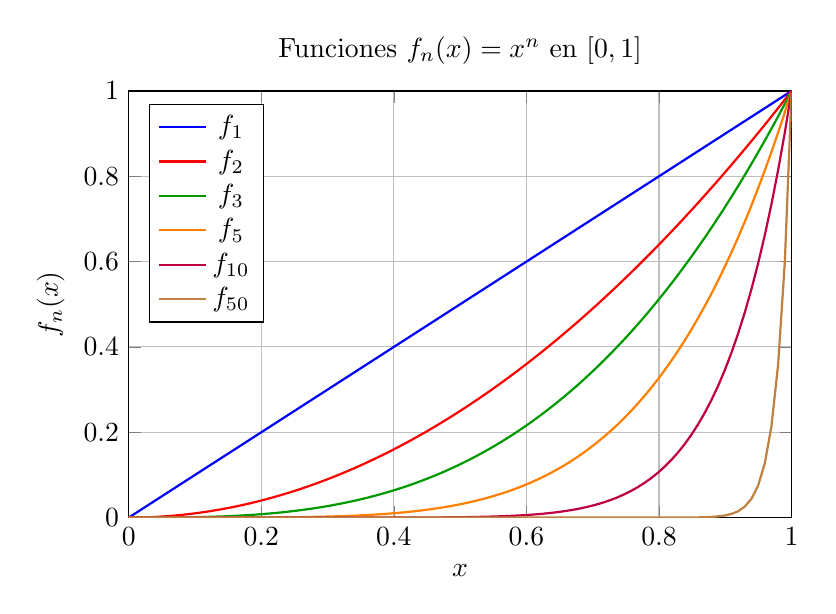
\begin{tikzpicture}
      \begin{axis}[
          width=10cm, height=7cm,
          xlabel={$x$},
          ylabel={$f_n(x)$},
          xmin=0, xmax=1,
          ymin=0, ymax=1,
          legend pos=north west,
          grid=major,
          title={Funciones $f_n(x) = x^n$ en $[0, 1]$}
        ]
        \addplot[domain=0:1, samples=100, thick, blue] {x^1};
        \addlegendentry{$f_1$}

        \addplot[domain=0:1, samples=100, thick, red] {x^2};
        \addlegendentry{$f_2$}

        \addplot[domain=0:1, samples=100, thick, green!60!black] {x^3};
        \addlegendentry{$f_3$}

        \addplot[domain=0:1, samples=100, thick, orange] {x^5};
        \addlegendentry{$f_5$}

        \addplot[domain=0:1, samples=100, thick, purple] {x^10};
        \addlegendentry{$f_{10}$}

        \addplot[domain=0:1, samples=100, thick, brown] {x^50};
        \addlegendentry{$f_{50}$}
      \end{axis}
    \end{tikzpicture}
  \end{center}
\end{eg}

\begin{eg}
  Las funciones $f_n\colon [0, 2\pi] \to \R$, $f_n(x) = \cos(nx)$, no convergen puntualmente: para $x = \pi$, $f_n(\pi) = {(-1)}^n$, que no tiene límite.
\end{eg}

Si $f_n\colon X \to \R$ converge puntualmente a $f$, para cada $\e > 0$ y cada $x \in X$ existe $n_0$ tal que $|f_n(x) - f(x)| < \e$ para todo $n > n_0$, pero $n_0$ depende de $\e$ y de $x$. Para $\e$ fijo puede ocurrir que ningún $n_0$ sirva para todo $x \in X$ a la vez.

\begin{eg}
  Sea $f_n(x) = x^n$ en $[0, 1]$, que converge puntualmente a la $f$ del ejemplo anterior. Para $\e = \frac{1}{2}$ y cada $n \in \N$, el punto $x = 2^{-1/n} \in [0, 1)$ cumple $|f_n(x) - f(x)| = x^n = \frac{1}{2} \geq \e$. Luego ningún $n_0$ sirve para todos los $x \in [0, 1)$ simultáneamente.
\end{eg}

\begin{definition}[Convergencia uniforme]
  La sucesión ${(f_n)}_{n \in \N}$ \emph{converge uniformemente} a $f\colon X \to \R$ si
  \[
    (\forall \e > 0)(\exists n_0 \in \N) \colon (\forall n > n_0)(\forall x \in X) \quad |f_n(x) - f(x)| < \e.
  \]
  Notamos $f_n \rightrightarrows f$.
\end{definition}

De la definición se deduce que $f_n \rightrightarrows f$ si y sólo si
\[
  \lim_{n \to +\infty} \sup_{x \in X} |f_n(x) - f(x)| = 0.
\]

\begin{eg}
  Por el ejemplo anterior, $f_n(x) = x^n$ no converge uniformemente en $[0, 1]$. Sea ahora $\delta \in (0, 1)$ y consideremos $f_n\colon [0, 1 - \delta] \to \R$; veamos que la convergencia a $f \equiv 0$ es uniforme. Para $x \in [0, 1 - \delta]$, $0 \leq x^n \leq {(1 - \delta)}^n$. Como $\lim_{n \to \infty} {(1 - \delta)}^n = 0$, dado $\e > 0$ existe $n_0$ con ${(1 - \delta)}^n < \e$ para $n > n_0$, y entonces $|x^n - 0| < \e$ para todo $n > n_0$ y todo $x \in [0, 1 - \delta]$.
\end{eg}

\begin{definition}[Sucesión de Cauchy de funciones]
  La sucesión ${(f_n)}_{n \in \N}$, con $f_n\colon X \to \R$, es \emph{de Cauchy} (uniformemente) si
  \[
    (\forall \e > 0)(\exists n_0 \in \N) \colon (\forall n, m > n_0)(\forall x \in X) \quad |f_n(x) - f_m(x)| < \e.
  \]
\end{definition}

\begin{theorem}
  Una sucesión de funciones $f_n\colon X \to \R$ converge uniformemente si y sólo si es de Cauchy.
\end{theorem}

\begin{proof}
  ($\Rightarrow$) Sea $f_n \rightrightarrows f$ y $\e > 0$. Existe $n_0$ tal que $|f_n(x) - f(x)| < \frac{\e}{2}$ para $n > n_0$ y todo $x \in X$. Si $n, m > n_0$,
  \[
    |f_n(x) - f_m(x)| \leq |f_n(x) - f(x)| + |f(x) - f_m(x)| < \e \qquad (\forall x \in X).
  \]

  ($\Leftarrow$) Para cada $x \in X$, ${(f_n(x))}_{n \in \N}$ es de Cauchy en $\R$, y por lo tanto converge; llamamos $f(x)$ a su límite. Dado $\e > 0$, existe $n_0$ tal que $|f_n(x) - f_m(x)| < \e$ para $n, m > n_0$ y todo $x \in X$. Fijando $x$ y $n > n_0$ y haciendo $m \to +\infty$ se obtiene $|f_n(x) - f(x)| \leq \e$ para todo $n > n_0$ y todo $x \in X$. Luego $f_n \rightrightarrows f$.
\end{proof}

Una serie de funciones $\sum f_n$ es un caso particular: sea $S_n = f_1 + \cdots + f_n$ la suma parcial. Decimos que $\sum f_n$ converge puntual o uniformemente a $f$ si $S_n$ lo hace, y en ese caso escribimos $\sum f_n \rightrightarrows f$. Por el teorema anterior, $\sum f_n$ converge uniformemente si y sólo si
\[
  (\forall \e > 0)(\exists n_0 \in \N) \colon (\forall n > n_0)(\forall p \in \N)(\forall x \in X) \quad |S_{n+p}(x) - S_n(x)| < \e.
\]

\begin{definition}[Convergencia normal]
  Decimos que una serie $\sum f_n$, con $f_n\colon X \to \R$, \emph{converge normalmente} si existe una sucesión ${(a_n)}_{n \in \N} \subset [0, +\infty)$ con $\sum a_n < +\infty$ y $|f_n(x)| \leq a_n$ para todo $n \in \N$ y todo $x \in X$.
\end{definition}

\begin{eg}
  La serie $\sum_{n \geq 1} \frac{\sin(nx)}{n^2}$ converge normalmente en $\R$, pues $\left| \frac{\sin(nx)}{n^2} \right| \leq \frac{1}{n^2}$ para todo $n$ y $\sum \frac{1}{n^2}$ converge.
\end{eg}

\begin{theorem}[Criterio de Weierstrass]
  Si $\sum f_n$ converge normalmente, entonces $\sum f_n$ y $\sum |f_n|$ convergen uniformemente.
\end{theorem}

\begin{proof}
  Sea $\e > 0$. Como $\sum a_n$ converge, por el criterio de Cauchy existe $n_0$ tal que $a_{n+1} + \cdots + a_{n+p} < \e$ para todo $n > n_0$ y todo $p \in \N$. Entonces, para todo $x \in X$,
  \begin{multline*}
    |S_{n+p}(x) - S_n(x)| = |f_{n+1}(x) + \cdots + f_{n+p}(x)| \\
    \leq |f_{n+1}(x)| + \cdots + |f_{n+p}(x)| \leq a_{n+1} + \cdots + a_{n+p} < \e.
  \end{multline*}
  Luego $\sum f_n$ converge uniformemente; el argumento para $\sum |f_n|$ es el mismo.
\end{proof}

La convergencia normal implica la convergencia uniforme, que a su vez implica la convergencia puntual, pero las recíprocas no valen.

\begin{eg}
  Sea $f_n\colon [1, +\infty) \to \R$ dada por
  \[
    f_n(x) = \begin{cases}
      \dfrac{1}{x} & \text{si } x \in [n, n + 1), \\[1ex]
      0            & \text{en caso contrario,}
    \end{cases}
  \]
  y sea $f(x) = \frac{1}{x}$. Afirmamos que $\sum_{n \geq 1} f_n \rightrightarrows f$. En efecto, $S_n(x) = \frac{1}{x}$ si $x \in [1, n + 1)$ y $S_n(x) = 0$ si $x \geq n + 1$. Luego $f(x) - S_n(x) = 0$ si $x < n + 1$, y $f(x) - S_n(x) = \frac{1}{x} \leq \frac{1}{n + 1} < \frac{1}{n}$ si $x \geq n + 1$; así, $0 \leq f - S_n < \frac{1}{n}$ en $[1, +\infty)$.

  Pero la serie no converge normalmente: si $|f_n(x)| \leq a_n$ para todo $x$, tomando $x = n$ resulta $a_n \geq \frac{1}{n}$, y $\sum a_n = +\infty$.
\end{eg}

\begin{note}
  Dada una sucesión ${(f_n)}_{n \in \N}$, nos preguntamos si los límites en $x$ y en $n$ pueden intercambiarse. En general, la respuesta es negativa.
\end{note}

\begin{eg}
  Sean $f_n(x) = x^n$ en $[0, 1]$ y $f$ su límite puntual. Entonces
  \begin{align*}
    \lim_{x \to 1} \left( \lim_{n \to \infty} f_n(x) \right) & = \lim_{x \to 1} f(x) = 0, \\
    \lim_{n \to \infty} \left( \lim_{x \to 1} f_n(x) \right) & = \lim_{n \to \infty} 1 = 1.
  \end{align*}
\end{eg}

\begin{theorem}
  Sea $a$ un punto de acumulación de $X \subset \R$ (o $a = \pm\infty$). Si $f_n \rightrightarrows f$ en $X$ y para cada $n \in \N$ existe $L_n = \lim_{x \to a} f_n(x)$, entonces existe $L = \lim_{n \to \infty} L_n$ y $\lim_{x \to a} f(x) = L$. Es decir,
  \[
    \lim_{n \to \infty} \left( \lim_{x \to a} f_n(x) \right) = \lim_{x \to a} \left( \lim_{n \to \infty} f_n(x) \right).
  \]
\end{theorem}

\begin{proof}
  Veamos primero que ${(L_n)}$ es de Cauchy. Dado $\e > 0$, existe $n_0$ tal que $|f_n(x) - f_m(x)| < \frac{\e}{3}$ para $n, m > n_0$ y todo $x \in X$. Fijemos $n, m > n_0$. Como $f_n(x) \to L_n$ y $f_m(x) \to L_m$ cuando $x \to a$, y $a$ es de acumulación, existe $x \in X$ tal que $|f_n(x) - L_n| < \frac{\e}{3}$ y $|f_m(x) - L_m| < \frac{\e}{3}$. Entonces
  \[
    |L_n - L_m| \leq |L_n - f_n(x)| + |f_n(x) - f_m(x)| + |f_m(x) - L_m| < \e.
  \]
  Luego ${(L_n)}$ converge a un $L \in \R$.

  Veamos ahora que $\lim_{x \to a} f(x) = L$. Dado $\e > 0$, existen $n_1$ con $|f_n(x) - f(x)| < \frac{\e}{3}$ para $n > n_1$ y todo $x \in X$, y $n_2$ con $|L_n - L| < \frac{\e}{3}$ para $n > n_2$. Sea $n > \max\{n_1, n_2\}$. Como $f_n(x) \to L_n$ cuando $x \to a$, existe $\delta > 0$ tal que $0 < |x - a| < \delta$ implica $|f_n(x) - L_n| < \frac{\e}{3}$. Para tales $x$,
  \[
    |f(x) - L| \leq |f(x) - f_n(x)| + |f_n(x) - L_n| + |L_n - L| < \e.
  \]
  Si $a = \pm\infty$, la demostración es la misma reemplazando la condición $0 < |x - a| < \delta$ por $x > R$ (o $x < -R$).
\end{proof}

\begin{corollary}
  Sea $a$ un punto de acumulación de $X$. Si $\sum f_n \rightrightarrows f$ en $X$ y para cada $n$ existe $L_n = \lim_{x \to a} f_n(x)$, entonces $\sum L_n$ converge y $\sum L_n = \lim_{x \to a} f(x)$. Es decir,
  \[
    \lim_{x \to a} \left( \sum f_n(x) \right) = \sum \left( \lim_{x \to a} f_n(x) \right).
  \]
\end{corollary}

\begin{proof}
  Se aplica el teorema a las sumas parciales $S_n$, que convergen uniformemente a $f$ y tienen $\lim_{x \to a} S_n(x) = L_1 + \cdots + L_n$.
\end{proof}

\begin{theorem}
  Sean $f_n\colon X \to \R$ funciones continuas en $a \in X$ tales que $f_n \rightrightarrows f$. Entonces $f$ es continua en $a$.
\end{theorem}

\begin{proof}
  Si $a$ es aislado en $X$, $f$ es continua en $a$ trivialmente. Si $a \in X'$, por continuidad $\lim_{x \to a} f_n(x) = f_n(a)$ para cada $n$, y por el teorema anterior,
  \[
    \lim_{x \to a} f(x) = \lim_{n \to \infty} f_n(a) = f(a). \qedhere
  \]
\end{proof}

En particular, si las $f_n$ son continuas pero el límite puntual no lo es, la convergencia no es uniforme. Por otro lado, que el límite sea continuo no alcanza para que la convergencia sea uniforme: $f_n(x) = x^n$ converge puntualmente a $0$ en $[0, 1)$, pero no uniformemente.

\begin{definition}[Convergencia monótona]
  Decimos que ${(f_n)}_{n \in \N}$ \emph{converge monótonamente} a $f$ si para todo $x \in X$ la sucesión ${(f_n(x))}_{n \in \N}$ es monótona y $f_n(x) \to f(x)$.
\end{definition}

\begin{theorem}[Dini]
  Sea $X \subset \R$ compacto. Si una sucesión de funciones continuas $f_n\colon X \to \R$ converge monótonamente a una función continua $f\colon X \to \R$, entonces la convergencia es uniforme.
\end{theorem}

\begin{proof}
  Dado $\e > 0$ definimos $K_n = \{ x \in X : |f_n(x) - f(x)| \geq \e \}$. Como $|f_n - f|$ es continua, $K_n$ es cerrado relativo a $X$, y por lo tanto compacto. Para cada $x$, como ${(f_n(x))}$ es monótona y converge a $f(x)$, la sucesión ${\bigl( |f_n(x) - f(x)| \bigr)}_n$ es decreciente, de modo que $K_1 \supset K_2 \supset K_3 \supset \cdots$. Además $\bigcap_{n} K_n = \varnothing$, pues si $x$ pertenece a todos los $K_n$, entonces $|f_n(x) - f(x)| \geq \e$ para todo $n$, lo que contradice $f_n(x) \to f(x)$.

  Supongamos que $K_n \neq \varnothing$ para todo $n$. Elegimos $x_n \in K_n$. Como $X$ es compacto, existe una subsucesión $x_{h(k)} \to x \in X$. Para cada $m$ fijo, $x_{h(k)} \in K_{h(k)} \subset K_m$ para $k$ grande, y como $K_m$ es cerrado relativo a $X$, $x \in K_m$. Entonces $x \in \bigcap_m K_m = \varnothing$, absurdo.

  Luego existe $n_0$ con $K_{n_0} = \varnothing$, y entonces $K_n = \varnothing$ para $n \geq n_0$, es decir, $|f_n(x) - f(x)| < \e$ para $n \geq n_0$ y todo $x \in X$.
\end{proof}

\begin{corollary}
  Sea $X \subset \R$ compacto y $f_n\colon X \to \R$ funciones continuas no negativas tales que $\sum f_n(x)$ converge para todo $x \in X$. Entonces $\sum f_n$ converge uniformemente si y sólo si su suma es continua.
\end{corollary}

\begin{proof}
  ($\Rightarrow$) Es el teorema de continuidad del límite uniforme. ($\Leftarrow$) Las sumas parciales $S_n = f_1 + \cdots + f_n$ son continuas y forman una sucesión creciente, pues las $f_n$ son no negativas, que converge puntualmente a una función continua. Por el teorema de Dini, la convergencia es uniforme.
\end{proof}

\section{Integración de sucesiones de funciones}

\begin{theorem}
  Si $f_n\colon [a, b] \to \R$ son integrables y $f_n \rightrightarrows f$, entonces $f$ es integrable y
  \[
    \int_a^b f(x) \,\dd x = \lim_{n \to +\infty} \int_a^b f_n(x) \,\dd x.
  \]
\end{theorem}

\begin{proof}
  Como las $f_n$ son acotadas y $f_n \rightrightarrows f$, $f$ es acotada. Sea $\e > 0$ y sea $\eta = \frac{\e}{4(b - a)}$. Existe $n$ con $|f_n(x) - f(x)| < \eta$ para todo $x \in [a, b]$. En cada subintervalo $[t_{i-1}, t_i]$ de una partición $P$ se tiene entonces $\omega_i(f) \leq \omega_i(f_n) + 2\eta$, de modo que
  \[
    S(f, P) - s(f, P) \leq S(f_n, P) - s(f_n, P) + 2\eta (b - a).
  \]
  Como $f_n$ es integrable, existe $P$ con $S(f_n, P) - s(f_n, P) < \frac{\e}{2}$, y entonces $S(f, P) - s(f, P) < \frac{\e}{2} + \frac{\e}{2} = \e$. Luego $f$ es integrable.

  Ahora, dado $\e > 0$ existe $n_0$ tal que $|f_n(x) - f(x)| < \frac{\e}{b - a}$ para $n > n_0$ y todo $x \in [a, b]$. Para esos $n$,
  \[
    \left| \int_a^b f \,\dd x - \int_a^b f_n \,\dd x \right| \leq \int_a^b |f - f_n| \,\dd x \leq \frac{\e}{b - a} (b - a) = \e. \qedhere
  \]
\end{proof}

\begin{corollary}
  Si $\sum f_n \rightrightarrows f$ en $[a, b]$ y las $f_n$ son integrables, entonces $f$ es integrable y $\int_a^b \sum f_n = \sum \int_a^b f_n$. Es decir, la serie puede integrarse término a término.
\end{corollary}

\begin{note}
  Si $f_n\colon [a, b] \to \R$ son integrables y convergen puntualmente a $f$, puede ocurrir que $f$ no sea integrable. Por ejemplo, si $\Q \cap [a, b] = \{ r_1, r_2, \dots \}$ y
  \[
    f_n(x) = \begin{cases}
      1 & \text{si } x \in \{ r_1, \dots, r_n \}, \\
      0 & \text{en caso contrario,}
    \end{cases}
  \]
  entonces $f_n \to f$ puntualmente, con $f(x) = 1$ si $x \in \Q \cap [a, b]$ y $f(x) = 0$ en caso contrario. Cada $f_n$ es integrable (tiene finitas discontinuidades), pero $f$ no lo es.
\end{note}

\begin{note}
  Aun cuando $f_n$ y $f$ sean integrables y $f_n \to f$ puntualmente, puede ser $\lim_{n \to \infty} \int_a^b f_n \neq \int_a^b f$. Por ejemplo, sea $f_n\colon [0, 1] \to \R$ dada por $f_n(x) = (n + 1) x^n$ si $x \in [0, 1)$ y $f_n(1) = 0$. Entonces $f_n \to 0$ puntualmente y $\int_0^1 f_n(x) \,\dd x = 1$ para todo $n$, pero $\int_0^1 0 \,\dd x = 0$.
\end{note}
